\chapter*{Цель работы}
Изучение методики и технологии синтеза аппаратных устройств ускорения вычислений по описаниям на языках высокого уровня. 

В ходе лабораторной работы рассматривается маршрут проектирования устройств, представленных в виде синтаксических конструкций ЯВУ C/C++, изучаются принципы работы IDE Xilinx Vitis HLS и методика анализа и отладки устройств. В ходе работы необходимо разработать ускоритель вычислений по индивидуальному заданию, разработать код для тестирования ускорителя, реализовать ускоритель с помощью средств высоко-уровненного синтеза, выполнить его отладку.

\chapter*{Ход работы}

\section*{Вариант индивидуального задания}
Мой вариант -- 6.

На листинге 1 представлен исходный код индивидуального задания.
\begin{lstinputlisting}[caption=Исходный код индивидуального задания, 
	basicstyle=\footnotesize\ttfamily, frame=single,breaklines=true]{src/main.c}
\end{lstinputlisting}

\section*{Файлы функций ядра на основе индивидуального задания}
На листингах 2-5 представлен код функций ядра на основе индивидуального задания:

\begin{lstinputlisting}[caption=Код без изменений, 
	basicstyle=\footnotesize\ttfamily, frame=single,breaklines=true]{src/main.c}
\end{lstinputlisting}

\begin{lstinputlisting}[caption=Развернутый цикл, 
	basicstyle=\footnotesize\ttfamily, frame=single,breaklines=true]{src/unroll.c}
\end{lstinputlisting}

\begin{lstinputlisting}[caption=Конвейерное исполнение, 
	basicstyle=\footnotesize\ttfamily, frame=single,breaklines=true]{src/pipe.c}
\end{lstinputlisting}

\begin{lstinputlisting}[caption=Развернутый цикл и конвейерное исполнение, 
	basicstyle=\footnotesize\ttfamily, frame=single,breaklines=true]{src/pipeunroll.c}
\end{lstinputlisting}

\section*{Результаты работы приложения в режиме \newline Emulation-SW}
На рисунке 1 представлен результат работы программы приложения в режиме Emulation-SW.

\FloatBarrier
\begin{figure}[h]
	\begin{center}
		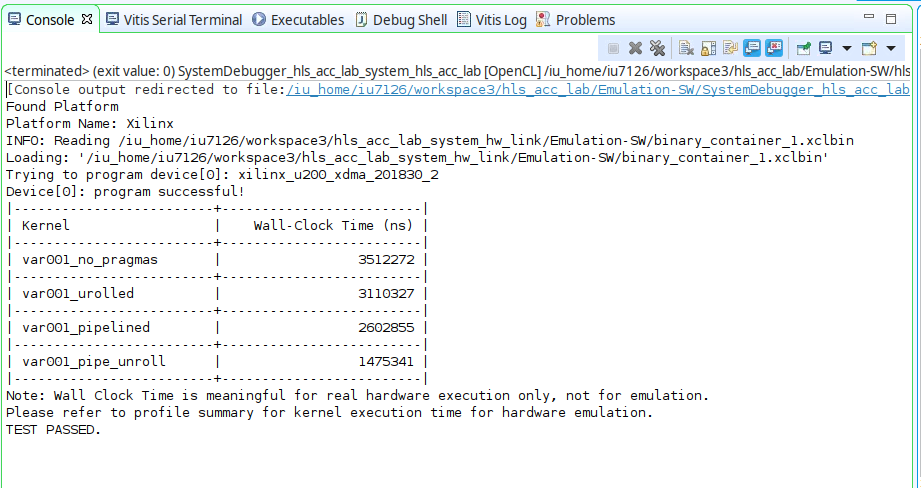
\includegraphics[width=\linewidth]{inc/emulationSWresult.png}
	\end{center}
	\caption{Результат работы программы приложения в режиме Emulation-SW}
\end{figure}
\FloatBarrier

Видно, что последующие оптимизации ускоряли работу программы.  
Оптимизация с помощью развёрнутого цикла и конвейерного выполнения показала лучшие результаты.
Это связано с тем, что итерации второго цикла могут быть выполнены параллельно, так как не зависят друг от друга.

\section*{Копия экрана Assistant View для \newline сборки Emulation-HW}
На рисунке 2 представлена копия экрана Assistant View для сборки Emulation-HW

\FloatBarrier
\begin{figure}[h]
	\begin{center}
		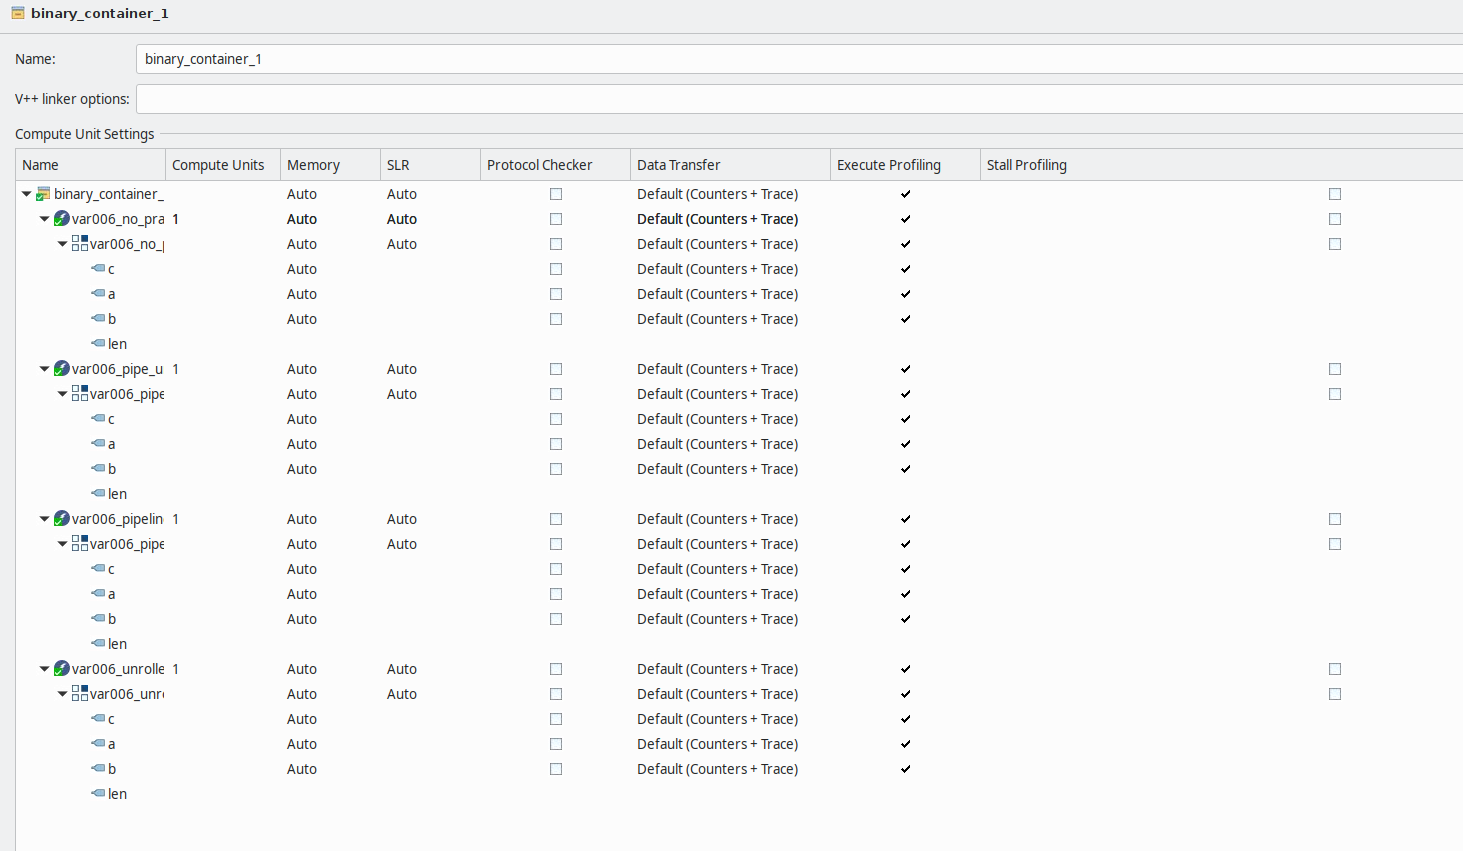
\includegraphics[width=\linewidth]{inc/assistant.png}
	\end{center}
	\caption{Копия экрана Assistant View для сборки Emulation-HW}
\end{figure}
\FloatBarrier

\section*{Результаты работы приложения в режиме \newline Emulation-HW}
Так как вывод оказался слишком большим, и на экран не поместился, результат выложен в виде листинга:

На листинге 6 представлен результат работы приложения в режиме Emulation-HW
\begin{lstinputlisting}[caption=Результат работы приложения в режиме Emulation-HW, 
	basicstyle=\footnotesize\ttfamily, frame=single,breaklines=true]{src/emulation-hw.txt}
\end{lstinputlisting}


Видно, что последующие оптимизации ускоряли работу программы.  
Оптимизация с помощью развёрнутого цикла и конвейерного выполнения показала лучшие результаты.
Это связано с тем, что итерации второго цикла могут быть выполнены параллельно, так как не зависят друг от друга.
\section*{Окно внутрисхемного отладчика Vivado для сборки в режиме Emulation-HW}
На рисунке 3 представлено окно внутрисхемного отладчика Vivado для сборки в режиме Emulation-HW

\FloatBarrier
\begin{figure}[h]
	\begin{center}
		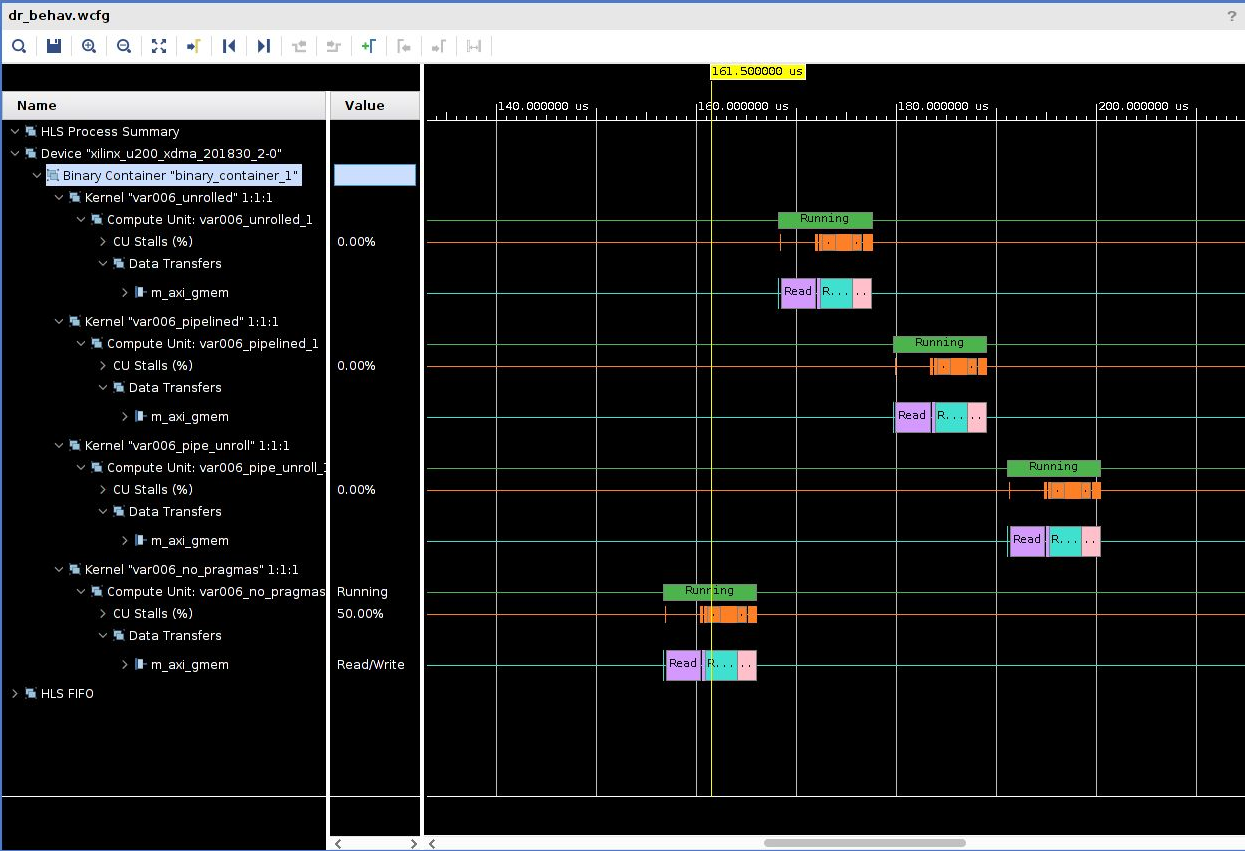
\includegraphics[width=\linewidth]{inc/vivado.png}
	\end{center}
	\caption{Окно внутрисхемного отладчика Vivado для сборки в режиме Emulation-HW}
\end{figure}
\FloatBarrier

\section*{Результаты работы приложения в режиме \newline Hardware}
На рисунке 4 представлены результаты работы приложения в режиме Hardware

\FloatBarrier
\begin{figure}[h]
	\begin{center}
		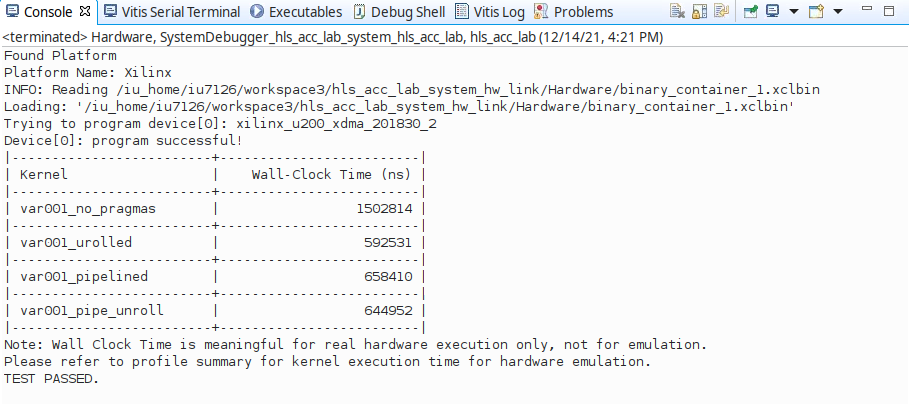
\includegraphics[width=\linewidth]{inc/hardware_result.png}
	\end{center}
	\caption{Результаты работы приложения в режиме Hardware}
\end{figure}
\FloatBarrier

Самым быстрым оказался вариант только с развёрнутым циклом, но все оптимизированные варианты тратят в 2.5 раза меньше тактов, чем стандартная программа.

\section*{Копия экрана для вкладок «Summary», \newline «System Diagram», «Platform Diagram» и четыре вкладки «HLS Synthesis» для каждого ядра \newline сборки Hardware.}

На рисунке 5 представлена копия экрана для вкладки Summary:

\FloatBarrier
\begin{figure}[h]
	\begin{center}
		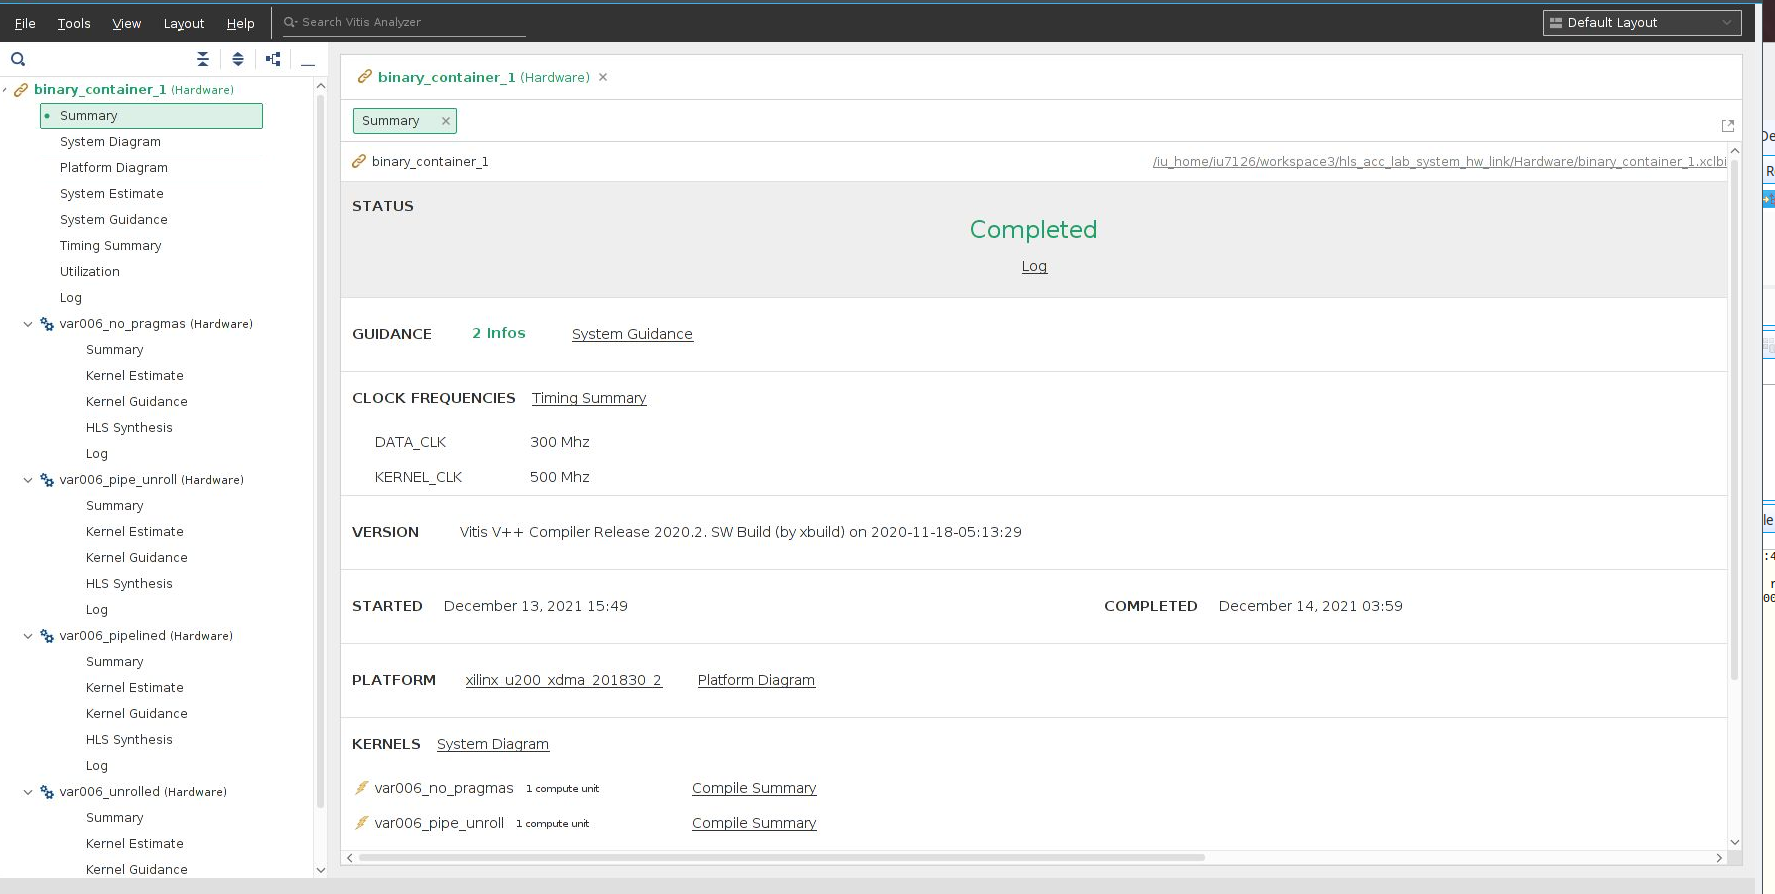
\includegraphics[width=\linewidth, height=8cm]{inc/summary.png}
	\end{center}
	\caption{Копия экрана для вкладки Summary}
\end{figure}
\FloatBarrier

На рисунке 6 представлена копия экрана для вкладки System Diagram:

\FloatBarrier
\begin{figure}[h]
	\begin{center}
		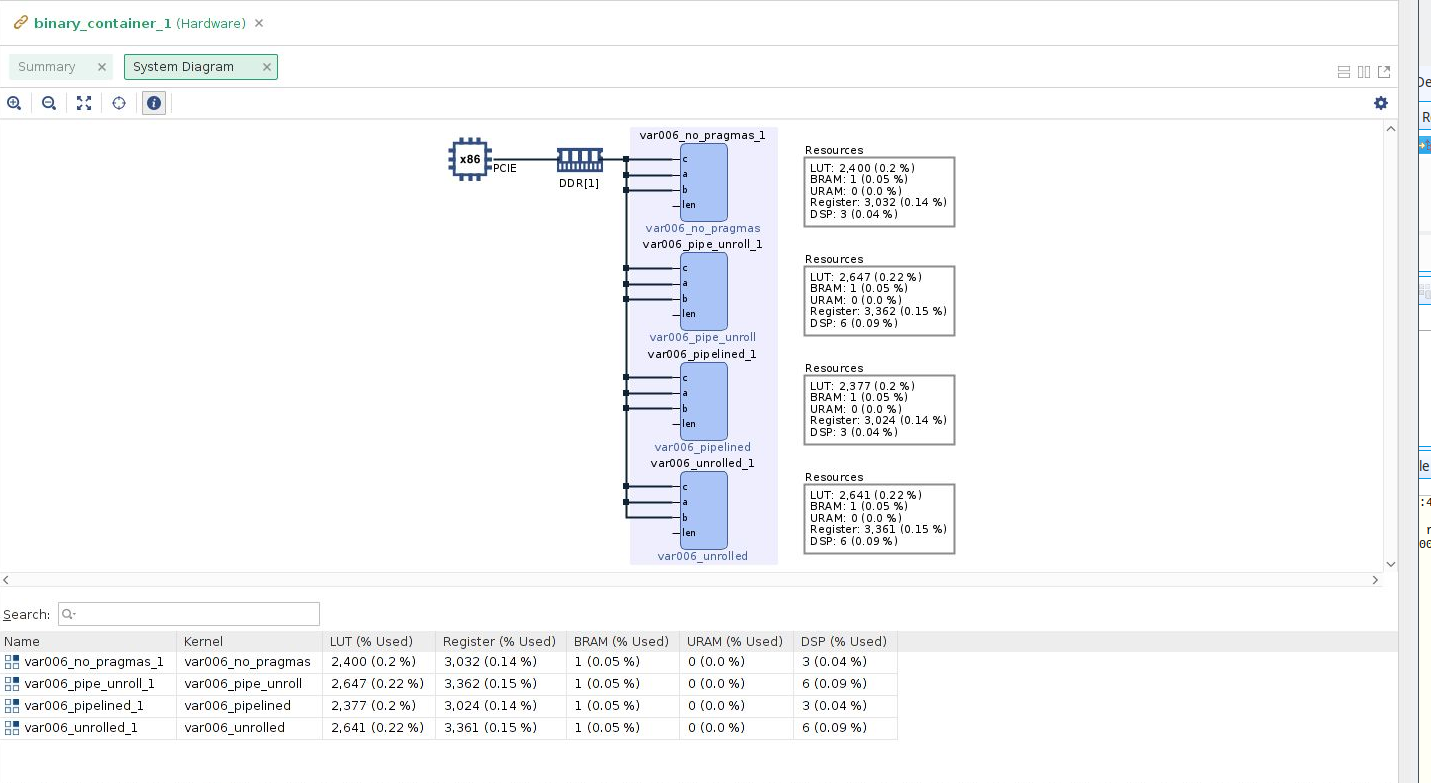
\includegraphics[width=\linewidth, height=8cm]{inc/sysdig.png}
	\end{center}
	\caption{Копия экрана для вкладки System Diagram}
\end{figure}
\FloatBarrier

На рисунке 7 представлена копия экрана для вкладки Platform Diagram:

\FloatBarrier
\begin{figure}[h]
	\begin{center}
		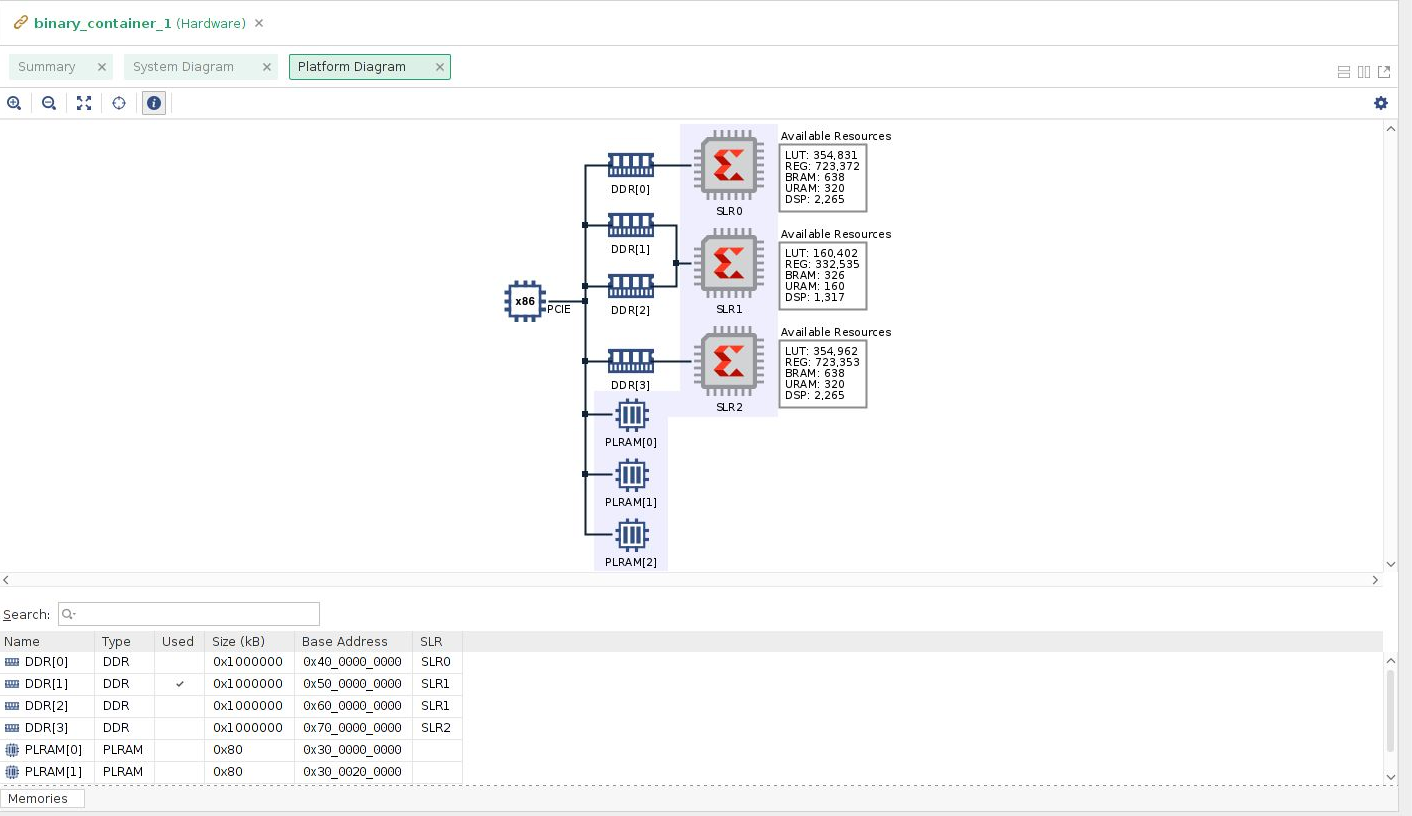
\includegraphics[width=\linewidth]{inc/pldig.png}
	\end{center}
	\caption{Копия экрана для вкладки Platform Diagram:}
\end{figure}
\FloatBarrier

На рисунке 8 представлена копия экрана для вкладки HLS Synthesis для ядра без оптимизаций
\FloatBarrier
\begin{figure}[h]
	\begin{center}
		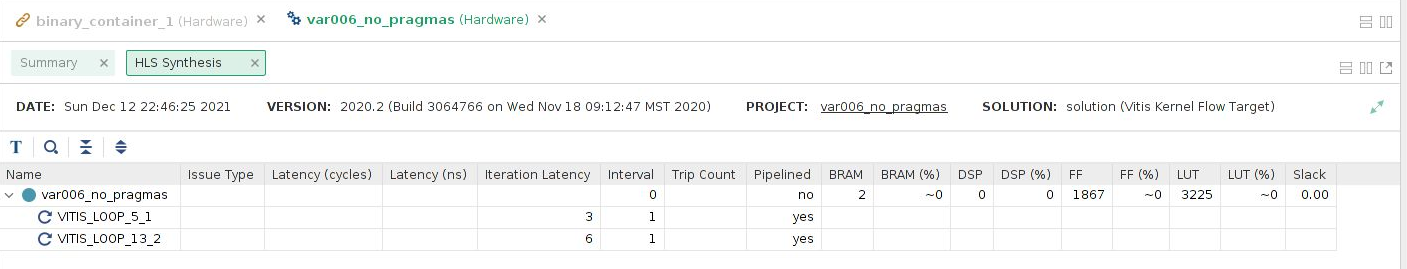
\includegraphics[width=\linewidth]{inc/hls1.png}
	\end{center}
	\caption{Копия экрана для вкладки HLS Synthesis для ядра без оптимизаций}
\end{figure}
\FloatBarrier

На рисунке 9 представлена копия экрана для вкладки HLS Synthesis для ядра с развёрнутым циклом:
\FloatBarrier
\begin{figure}[h]
	\begin{center}
		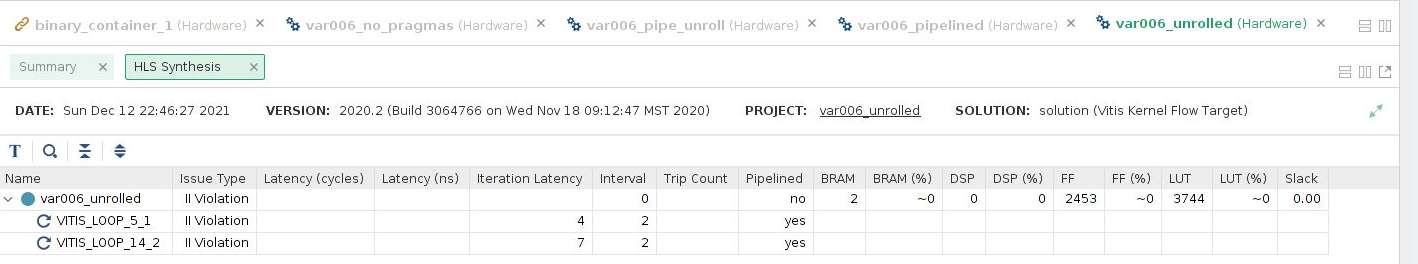
\includegraphics[width=\linewidth]{inc/hlsunroll.png}
	\end{center}
	\caption{Копия экрана для вкладки HLS Synthesis для ядра с развёрнутым циклом}
\end{figure}
\FloatBarrier

На рисунке 10 представлена копия экрана для вкладки HLS Synthesis для ядра с конвейерным выполнением:
\FloatBarrier
\begin{figure}[h]
	\begin{center}
		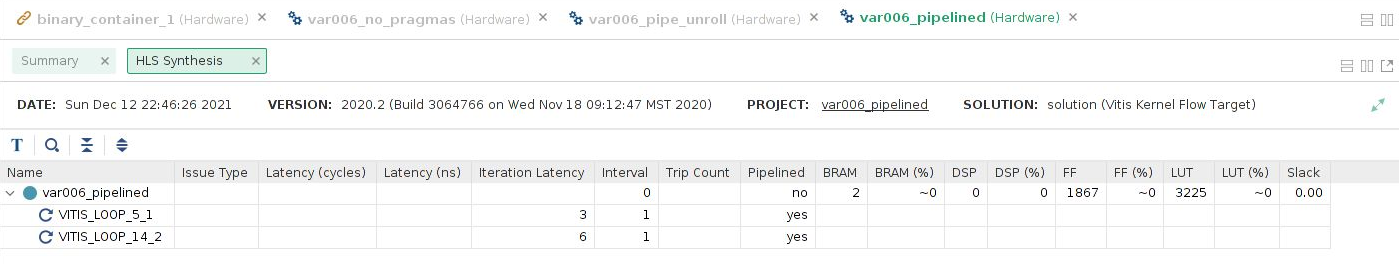
\includegraphics[width=\linewidth]{inc/hlspipe.png}
	\end{center}
	\caption{Копия экрана для вкладки HLS Synthesis для ядра с конвейерным выполнением}
\end{figure}
\FloatBarrier

На рисунке 11 представлена копия экрана для вкладки HLS Synthesis для ядра с развёрнутым циклом и конвейерным выполнением:
\FloatBarrier
\begin{figure}[h]
	\begin{center}
		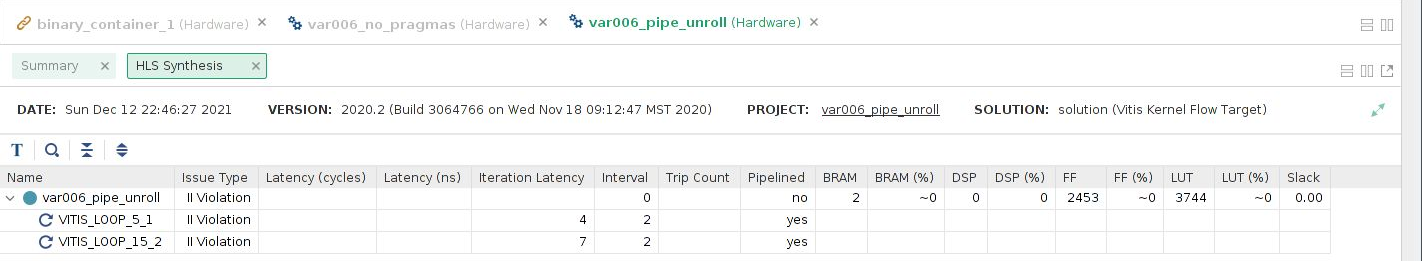
\includegraphics[width=\linewidth]{inc/hls2.png}
	\end{center}
	\caption{Копия экрана для вкладки HLS Synthesis для ядра с развёрнутым циклом и конвейерным выполнением}
\end{figure}
\FloatBarrier

\section*{Выводы}
В ходе лабораторной работы были изучены принципы работы IDE Xilinx Vitis HLS и методика анализа и отладки устройств. 
В ходе работы был разработан ускоритель вычислений по индивидуальному заданию, разработан код для тестирования ускорителя, реализован ускоритель с помощью средств высоко-уровненного синтеза, выполнена его отладку.

Удалось запустить приложение в трёх режимах: Emulation-SW, Emulation-HW и Hardware.
С помощью оптимизаций удалось значительно ускорить работу программы.
Для Emulation-SW и Emulation-HW быстрее всего отработала оптимизация с помощью развёрнутого цикла и конвейрного выполнения.
Для Hardware самым быстрым оказался вариант только с развёрнутым циклом, но все оптимизированные варианты тратят в 2.5 раза меньше тактов, чем стандартная программа.

Оптимизация стала возможна, потому что итерации второго цикла исходного кода могут быть выполнены параллельно, так как не зависят друг от друга.

